\section{Chapter Overview}
This chapter discusses how testing was carried out to ensure that functions flowed as expected. It will cover testing objectives and procedures such as model testing, benchmarking, functional testing, non-functional testing, module, and integration testing.

\section{Objectives and Goals of Testing}
The primary goal of software testing is to ensure that the system is performing as expected based on the requirements acquired.

These expectations can be broken down as follows
\begin{itemize}
\item Ensure that all models of the system are working as intended and that they have been tested in order to achieve the desired optimum results.
\item Ensure that the system meets the MoSCoW technique's mandatory "Must have" and "Should have" functional requirements.
\item Apply possible benchmarking techniques that can be used to benchmark the developed system for future work.
\item Identify if the required \& important non-functional requirements have been satisfied.
\item Identify possible points of improvements/ bug fixes that can be applied to the system.
\end{itemize}


\section{Testing Criteria}
With the goal of narrowing the gap between the intended and implemented systems, a criterion to test the system in two ways was defined. The following are the two methods for testing:
\begin{enumerate}
\item Functional Quality - This focuses on the system's development characteristics and technical requirements in order to see how well it meets the specified design based on functional requirements.
\item Structural Quality - This tests the system's non-functional requirements while ensuring that it meets the functional requirements' performance criteria.
\end{enumerate}


\section{Model Testing \& Evaluation}

\subsection{Model Testing}

% The content based recommender, trait rarity, trait content recommenders and trends-based recommenders 

The multiple ensemble models developed in the project were tested based on the following conditions.

% \vspace{-4mm}
\begin{longtable}[h!]{|l|p{0.65\linewidth}|}
\caption{Testing Trait Content \& Trait Rarity based recommendations}
\endfirsthead
\hline
\textbf{Model} & \textbf{Testing Method} \\
\hline
Trait Rarity based RecSys & The total rarity being as close as possible to the reference item's rarity\\
\hline
Trait Content based RecSys & Cosine Similarity being the closest to the reference item's traits\\
\hline
Trends based RecSys & Check if the items that get the highest trend score will be recommended and identify if the most trending, accepted \& timely items are obtained using the available data. \\
\hline
\end{longtable}

\noindent Following graphical analysis of the test output shows the validity of the outputs produced by the trait rarity \& content based models.


\begin{figure}[h!]
     \centering
     \begin{subfigure}[b]{0.45\textwidth}
         \centering
         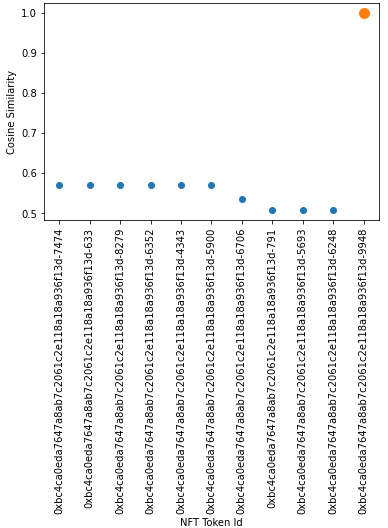
\includegraphics[width=\textwidth]{images/Testing/Cosine Similarities of Recommended NFTs - Trait Content Based Recomendations Model.png}
         \caption{Trait Content based recommendations}
         \label{fig:trait-content-output}
     \end{subfigure}
     \hfill
     \begin{subfigure}[b]{0.45\textwidth}
         \centering
         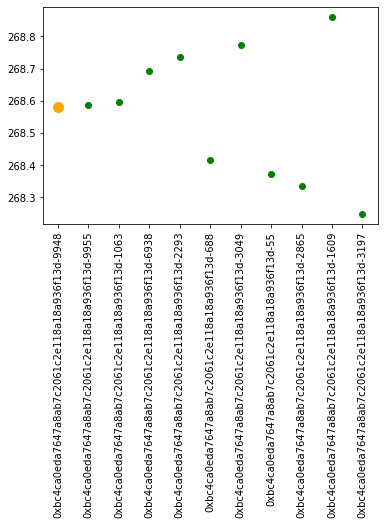
\includegraphics[width=\textwidth]{images/Testing/Trait rarity representation graph - rarity recommendations.png}
         \caption{Total Rarity based recommendations}
         \label{fig:total-rarity-output}
     \end{subfigure}
     \hfill
        \caption{Outputs produced by Trait Content \& Rarity Recommendation Systems \textit{(self-composed)}}
        \label{fig:trait-recs-outputs}
\end{figure}


% TODO: test this with multiple collections and add findings graphs to appendix



\subsection{Model Evaluation}

\subsubsection{Trait Rarity \& Content based Recommendations Systems}

% TODO: test if the closest 10 are obtained in both algorithms

The \gls{nft} trait rarity and trait content based Recommendation Systems were matched against each other to demonstrate the difference in recommendations produced by each other even though they are both generated based on the traits and overall repetition of each of these traits across a collection.

% \vspace{-4mm}
\begin{table}[h!]
\centering
\caption{Evaluating Trait Content \& Trait Rarity based recommendations}
\begin{tabular}{|l|l|l|l|}
\hline
\textbf{Testing Method} & \textbf{precision@k} &
\textbf{recall@k} & \textbf{f1\_score@k} \\
\hline
self-scored & 1.0 & 1.0 & 1.0 \\
\hline
combined-scored & 1.0 & 0.5 & 0.67\\
\hline
\end{tabular}
\end{table}

The above precision \& recall @k are customized precision \& recalls created for the purpose of testing \& evaluating Recommendations Systems.

These were calculated using the below formulae.

\[\text{Recommender System Precision} = \frac{\text{no. of recommendations that are relevant}}{\text{no. of items that we recommended}}\]

\[\text{Recommender System Recall} = \frac{\text{no. of recommendations that are relevant}}{\text{no. of all the possible relevant items}}\]

\noindent The formula for f1 score is the same, except that the above altered precision \& recall were used.

% TODO: discuss the results - why both precision & recall cannot be high in a recommendations system.

The reason that both the models were self-scored \& combined-scored was to demonstrate that although they produce the best possible results by themselves, using only one of the models won't give all the possible results. This can be further explained with the aggregate diversity graphs displayed in the \textbf{\nameref{sec:test-benchmarking}} section.

% show graphs with all outputs here - to explain why combined score is necessary to be considered & both models are important.
\begin{figure}[h!]
     \centering
     \begin{subfigure}[b]{0.45\textwidth}
         \centering
         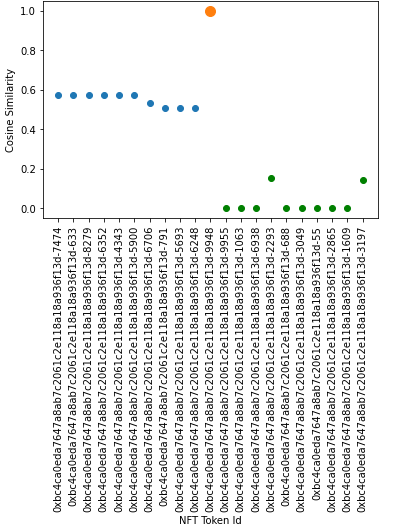
\includegraphics[width=\textwidth]{images/Testing/Cosine Similarities of Recommended NFTs (Trait Content Based + Total Rarity Recomendations Models).png}
         \caption{Cosine similarities of content}
         \label{fig:1-1}
     \end{subfigure}
     \hfill
     \begin{subfigure}[b]{0.45\textwidth}
         \centering
         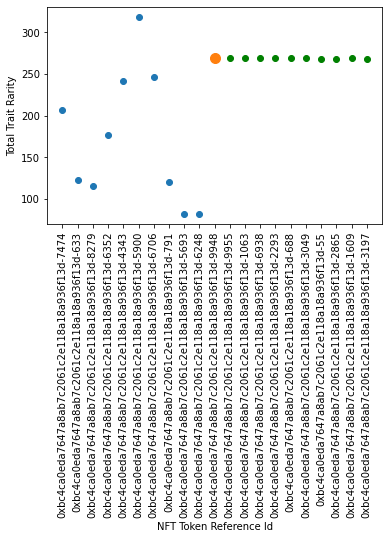
\includegraphics[width=\textwidth]{images/Testing/Total rarities content + rarity based.png}
         \caption{Total rarities}
         \label{fig:1-2}
     \end{subfigure}
     \hfill
        \caption{Comparison Recommendations generated by both models \textit{(self-composed)}}
        \label{fig:1}
\end{figure}

The above graphs establishes the necessity of generating recommendations from both models.

The items marked in blue were recommended by the Trait content based RecSys, the green ones by the Trait rarity based RecSys and the orange item was the reference item used to generate recommendations.
It is clear that although both the trait content and rarity based Recommendation Systems are generating recommendations using traits of items, they produce very different outputs, especially in the case of rarity based recommendations.


\subsubsection{Trends based Recommendations System}


The trends-based recommender that is expected to enhance content-based Recommendation Systems with Collaborative-filtering-like capabilities without collecting user click-data was tested to identify if the treds based recommendations were possible to be generated.


\begin{figure}[h!]
\centering
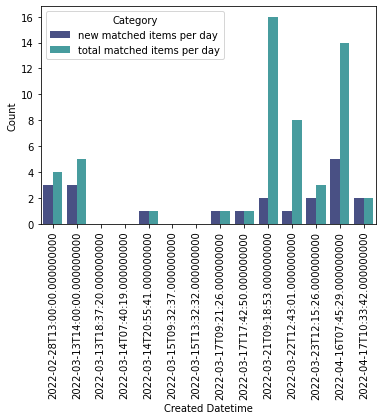
\includegraphics[width=0.6\textwidth]{images/Testing/trends-matches-eval1.png}
\caption{Evaluation of Trends based Recommender \textit{(self-composed)}}
\label{fig:trends-recsys-new-matches}
\end{figure}


\section{Benchmarking}
\label{sec:test-benchmarking}

% mention aggregate diversity of trait content & rarity based recommendations here.
% TODO: show aggregate diversity graph here. reference to the graphs in appendix?
The following graph shows the aggregate diversity of items generated by both the models by using the entire \textit{Bored Ape Yatch Club} \gls{nft} collection of 10,000 \gls{nft}s.

\begin{figure}[h!]
\centering
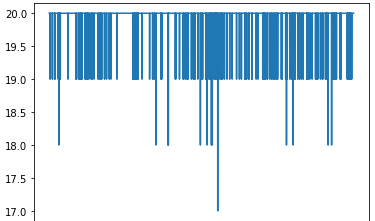
\includegraphics[width=0.7\textwidth]{images/Testing/aggregate diversity.png}
\caption{Aggregate diversity of generated Recommendations \textit{(self-composed)}}
\label{fig:aggregate-diversity-traits}
\end{figure}

\noindent As displayed, the maximum overlapping of items was 3, while most recommendations had 1 or less than one similarities.

% TODO: benchmark trends based recommender
% show using how many days/ trends, how many items were recommended out of the total number in the collection.
% Can show how the recommendations vary with time as well


\section{Functional Testing}
The application was functionally tested against the Functional Requirements (FR) specified during the requirements gathering phase.

% refer table in appendix?
\noindent\textit{\nameref{tab:test-func-requirements}} in \textbf{\nameref{appendix:testing}} shows the breakdown of functional tests that were carried out.

\section{Module \& Integration Testing}

% Data collection: trends fetching & nft data fetching modules

% trends scoring module

% sentiment analysis module
%  - explain why this model was chosen in the implementation chapter? or display outputs in appendix & explain here

\begin{longtable}{|p{0.18\textwidth}|p{0.2\textwidth}|p{0.2\textwidth}|p{0.2\textwidth}|l|} 
\hline
\textbf{Module} & \textbf{Input} & \textbf{Expected Output} & \textbf{Actual Output} & \textbf{Status} \endfirsthead 
\hline
Trends Data-fetcher & New raw Trends data & Extract required data and save & Extract required data and save & Passed \\ 
\hline
NFT Data-fetcher & NFT asset data & Filters out required information and calculates rarity score~ & Filtered out required information and calculates rarity score~ & Passed \\ 
\hline
Trends scorer & Trends with sentiment score, volume and trend datetime & Trend score & Trend score & Passed \\ 
\hline
Sentiment Analyzer & Top tweets of each trend & Sentiment score  sentiment polarity & Sentiment score  sentiment polarity & Passed \\
\hline
\end{longtable}

\section{Non-functional Testing}

% \subsection{Performance}

% \subsection{Security}

\subsection{Important Non-functional Requirement Completion Percentage}


\section{Limitations of Testing Process}

As an initial study of recommending \gls{nft}s, it was difficult to pin-point on the ground truth of what exactly should've been produced by the models as recommendations. 

With the trends based recommender, the unavailability of past trends data restricted extensive testing. The unavailability of an open e-commerce dataset restricted from benchmarking the models. The lack of data was the biggest constraint in testing, evaluating \& benchmarking this project.

\section{Chapter Summary}
This chapter covered extended testing, evaluation \& benchmarking of the core-research component. Furthermore functional, integration and non-functional tests were carried out \& the results were recorded. Any limitations of the process was explained at the end.